\chapter{Results}
\label{Results}
The result section is structured in two parts. Firstly, we highlight the empirical relationship between daily idiosyncratic volatility of the individual stocks and the resulting one-day-ahead return forecasting performance. Secondly, we pool the stocks in four equally sized, equally weighted portfolios by their constituent's daily IV percentage, and then assess the overall return forecasting performance of our defined portfolios.

\section{Individual stocks}

We commence our analysis by examining a pooled regression of the relationship between the daily IV percentage and the one-day-ahead squared forecast error for all the stocks over the whole period, visualized in figure \ref{Scatter regression}: 

\begin{figure}[h]
    \centering
    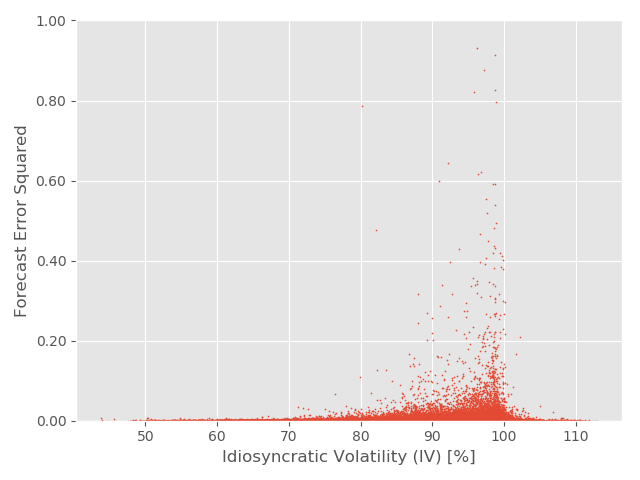
\includegraphics[scale = 0.5]{Plot/ScatterRegression.png}
    \caption{Regression: daily IV percentage on squared return forecasting error}
    \label{Scatter regression}
\end{figure}

Figure \ref{Scatter regression} indicate the existence of a positive relationship between the daily IV percentage and squared forecast error. Visually, one could also infer a weak positive exponential relationship. The result implies that it is more difficult to accurately and precisely predict tomorrows return for stocks with a high daily IV percentage.

Furthermore, we examine the relationship between the average daily IV percentage and the \textit{sign ratio}. Running a regression on each stock's average daily IV percentage and its sign ratio, we obtain the following plot: 

\begin{figure}[h]
    \centering
    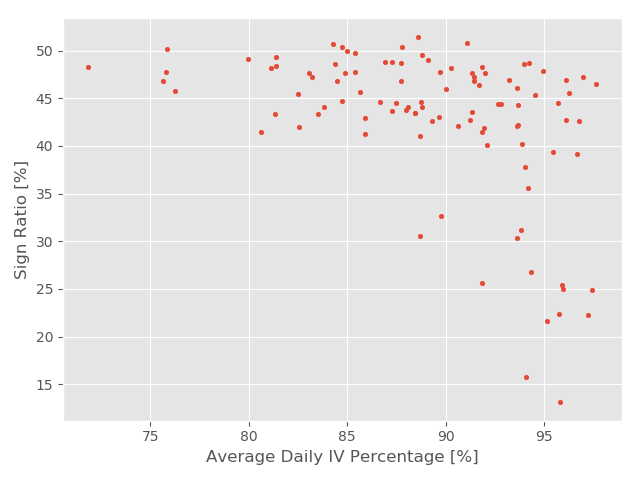
\includegraphics[scale = 0.5]{Plot/IndividualStockRegression1.png}
    \caption{Regression: average daily IV percentage on Sign error}
    \label{IVSignError}
\end{figure}

Figure \ref{IVSignError} visually illustrate that it's more difficult to predict the direction of the one-day-ahead return for stocks with a high average daily IV percentage. From table \ref{RegressionIndividualStocks} we confirm this by observing that we have a significant $\beta$ at $-0.319$. Like our observations in Figure \ref{Scatter regression}, one can visually infer a weak negative exponential relationship between sign ratio and average daily IV percentage.

So far the presented results have indicated that it is harder to predict the one-day-ahead return for stocks with a high average daily IV percentage, both in terms of accuracy, precision and direction. Now, we wish to examine the profitability of following the predictions of our return forecasting model. 

Therefore, we run a regression on each stock’s average daily IV percentage on the alpha, defined as the difference $r_{sign}-r_{economic}$. This yields a rather surprising result.

\begin{figure}[h]
    \centering
    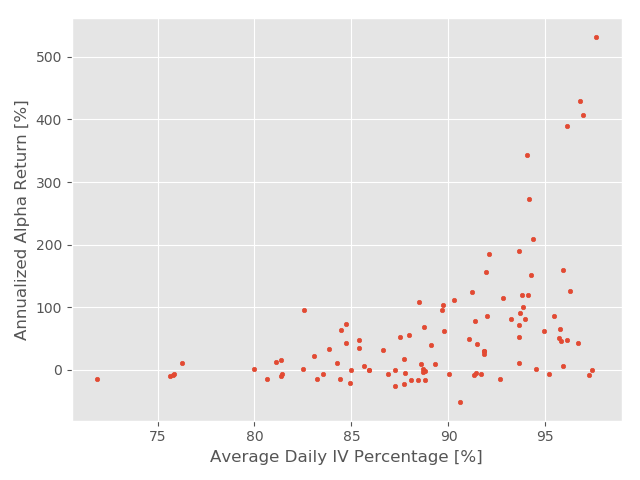
\includegraphics[scale = 0.5]{Plot/IndividualStockRegression2.png}
    \caption{Regression: average daily IV percentage on annualized alpha return}
    \label{IVAlphaRegression}
\end{figure}

\newpage

Figure \ref{IVAlphaRegression} illustrates that following the sign strategy generates a positive alpha for a majority of the stocks in the sample. Moreover, Table \ref{RegressionIndividualStocks} confirms the positive relationship between the daily average IV percentage and the alpha, with a significant $\beta$ of $0.003$. 

Figure \ref{IVtoVol}, shows the relationship between average daily IV percentage and annualized economic standard deviation:

\begin{figure}[h]
    \centering
    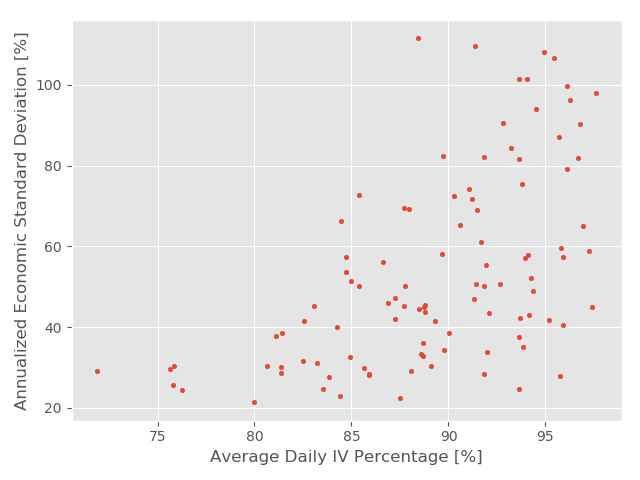
\includegraphics[scale = 0.5]{Plot/IVvsEconomicVolatilityRegression.png}
    \caption{Regression: average daily IV percentage on annualized economic standard deviation}
    \label{IVtoVol}
\end{figure}

Here we can observe the positive correlation between a high daily IV percentage and economic standard deviation. This emphasizes that stocks with a high average daily IV percentage also tend to exhibit a higher volatility.  

This leads to two preliminary interpretations: the return forecasting performance for the one-day-ahead return in terms of direction or accuracy, precision is worse for stocks with a high daily IV percentage. Also, the return forecasting model generates positive alpha for these stocks. This can understood by the fact these stocks tend to exhibit a higher total volatility and the return forecasting model seems to predict the bigger directional movements when volatility, and hence daily IV percentage, is greater.

Table \ref{RegressionIndividualStocks} below shows the results and parameters of the four regressions presented in this section:

\newcolumntype{P}[1]{>{\centering\arraybackslash}p{#1}}
%\begin{landscape}
\begin{longtable}{P{2cm}P{2cm}P{2cm}P{2cm}P{2cm}P{2cm}P{2cm}} 
\caption{Regression Individual Stocks}
\label{RegressionIndividualStocks}\\
\hline
\textbf{Figure} & \textbf{Observations} & \textbf{Adj. }$\boldsymbol{R^{2}}$ & \textbf{Intercept} & \textbf{P-Value} & \textbf{Beta} & \textbf{P-Value} \\
\hline
\endfirsthead
\multicolumn{7}{c}%
{\tablename\ \thetable\ -- \textit{Continued from previous page}} \\
\hline
\textbf{Figure} & \textbf{Observations} & \textbf{Adj. }$\boldsymbol{R^{2}}$ & \textbf{Intercept} & \textbf{P-Value} & \textbf{Beta} & \textbf{P-Value} \\
\hline
\endhead
\hline \multicolumn{7}{r}{\textit{Continued on next page}} \\
\endfoot
\hline
\endlastfoot
\input{Input/RegressionTable.txt}
\end{longtable}
%\end{landscape}

For more detailed results on the individual stocks, the reader is referenced to Appendix A.

\section{Equally sized, equally weighted portfolios}

In the previous section, we looked at the empirical relationship between individual stocks' daily IV proportion and return forecasting performance. In this section, we pool stocks in four equally sized, equally weighted portfolios by their constituents daily IV percentage, and discuss the overall return forecasting performance by assessing the portfolios return, sign ratio and Sharpe ratio. By pooling companies into portfolios we obtain diversification benefits, differences in the relationship between individual stocks' average daily IV proportion and their return forecasting performance are evened out. As a result, using portfolios instead of individual stocks, we are able to identify a clearer relationship between IV proportion and return forecasting performance. 

Our findings are presented in Table \ref{Portfolio Metrics}. The first column denotes the portfolio number. The second column is the average daily IV percentage. Column three and four denotes the annualized economic return and the annualized standard deviation of the economic return, respectively. Column six denotes the sign ratio, and column seven and eight denotes the annualized sign return and the annualized standard deviation of the sign return, respectively. In column nine the annualized alpha is denoted. The mean of the annualized daily forecast errors, the annualized daily accuracy, is denoted in column ten. The annualized RMSE of the daily forecast errors, the annualized daily precision, is denoted in column eleven. Finally, in column twelve and thirteen, we find the Sharpe ratio of the annualized economic return and annualized sign return, respectively. 

Our findings in Table \ref{Portfolio Metrics} shows that equally sized, equally weighted portfolios with higher average daily IV percentage generates higher annualized economic returns on average, than equally sized, equally weighted portfolios with lower average daily IV percentage. This result is not directly related to forecasting performance, but is still an interesting observation, as it supports the conclusions of Østnes and Hafskjær \cite{ostnes}. However, this is in contrast to the low idiosyncratic volatility anomaly introduced by Ang et al. \cite{angetal06}, supported in the Norwegian Stock Market concluded by Arnesen and Borge \cite{arnborge} and Tjaum and Wiedswang \cite{thaumwiedswang}. Arnesen and Borge \cite{arnborge} and Tjaum and Wiedswang \cite{thaumwiedswang} get the same results with both equally weighted and market weighted portfolios. However, they do not operate in an daily rebalanced environment as we do in this paper, which may give quite different results considering that that daily financial data contains short-term noise. Looking at the evidence presented in Appendix B, it reasonable to assume that a market weighted portfolio would result in similar annualized economic returns as Arnesen and Borge \cite{arnborge} and Tjaum and Wiedswang \cite{thaumwiedswang}. 

Furthermore, we find that portfolios with higher average daily IV percentage has higher mean forecast error. Not only does it exist a positive relationship between average daily IV percentage and the annualized mean forecast error, the forecast errors also have higher annualized RMSE as the average daily IV percentage increases. Furthermore, as the average daily IV percentage increases, the sign ratio decreases. In other words, it seems harder to predict both the magnitude and direction of the one-day-ahead return for the portfolios with high average daily IV percentage. To, conclude, we have found a negative relationship between average daily IV percentage and forecast performance of the portfolios in terms of accuracy, precision and direction. 

Despite the negative relationship between average daily IV percentage and forecast performance of the portfolios in terms of accuracy, precision and direction, the annualized alpha increases as the average daily IV increases. Our findings suggest that portfolios with a higher average daily IV percentage also tend to have higher economic standard deviation. Hence, a reason for the increase in alpha, despite the negative relationship between average daily IV percentage and forecast performance of the portfolios in terms of accuracy, precision and direction, might be that it is easier for the return return forecasting model to predict the bigger directional movements when economic standard volatility, and hence average daily IV percentage, is greater. In other words, each correct prediction generates a high magnitude return despite it happens more infrequently as the average daily IV percentage increases

Another interesting observation is that the annualized economic standard deviation decreases, as the average daily IV percentage increases, despite the increase in annualized economic return. Consequently, the diversification effect is greater in equally weighted portfolios containing stocks with a high proportion of IV, even though we showed a positive correlation between a high daily IV percentage and annualized economic standard deviation in the last section. This is reasonable considering that diversification is about reducing the idiosyncratic volatility.

Our findings also suggest that the annualized standard deviation of the sign return is less compared to the annualized standard deviation of the economic return, for all four portfolios. The difference between the annualized standard deviations are greater for portfolios with lower average daily IV percentage. A greater annualized sign return combined with a lower annualized sign standard deviation, implies a Sharpe ratio that is greater than the Sharpe ratio of the annualized economic return. 

Taking into account that the return forecasting model trades on every stock in each equally weighted portfolio every day and does not incorporate transaction costs, the annualized sign return, and hence the Sharpe ratio, is expected to be less than calculated in Table \ref{Portfolio Metrics}. See Appendix C for the development of the returns for each of the four portfolios. 

\newcolumntype{P}[1]{>{\centering\arraybackslash}p{#1}}
\begin{landscape}
\begin{longtable}{P{1.5cm}P{1.5cm}P{1.5cm}P{1.5cm}P{1.6cm}P{1.5cm}P{1.5cm}P{1.5cm}P{1.5cm}P{1.5cm}P{1.5cm}P{1.5cm}} 
\caption{Portfolio Metrics: Sorted by increasing average daily IV percentage}
\label{Portfolio Metrics}\\
\hline
\textbf{Portfolio} &  \textbf{Daily }$\boldsymbol{\bar{IV}}$\textbf{ }& $\boldsymbol{r_{economic}}$ & $\boldsymbol{\sigma_{economic}}$ & \textbf{Sign Ratio} &  $\boldsymbol{r_{sign}}$ & $\boldsymbol{\sigma_{sign}}$ & $\boldsymbol{\alpha}$ & $\boldsymbol{\bar\epsilon_{forecast}}$ & $\boldsymbol{RMSE}$ & $\boldsymbol{S_{economic}} $ & $\boldsymbol{S_{sign}}$ \\
\hline
\endfirsthead
\multicolumn{12}{c}%
{\tablename\ \thetable\ -- \textit{Continued from previous page}} \\
\hline
\textbf{Portfolio} & \textbf{Daily }$\boldsymbol{\bar{IV}}$\textbf{ } & $\boldsymbol{r_{economic}}$ & $\boldsymbol{\sigma_{economic}}$ & \textbf{Sign Ratio} &  $\boldsymbol{r_{sign}}$ & $\boldsymbol{\sigma_{sign}}$ & $\boldsymbol{\alpha}$ & $\boldsymbol{\bar\epsilon_{forecast}}$ & $\boldsymbol{RMSE}$ & $\boldsymbol{S_{economic}} $ & $\boldsymbol{S_{sign}}$ \\
\hline
\endhead
\hline \multicolumn{12}{r}{\textit{Continued on next page}} \\
\endfoot
\hline
\endlastfoot
\input{Input/PortfolioTable.txt}
\end{longtable}
\end{landscape}
